\begin{center}
\begin{minipage}[t]{.46\linewidth}\vspace{0pt}\centering
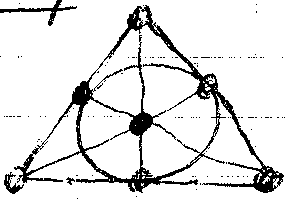
\includegraphics[width=\linewidth]{figures/gelfand-0153-p001411-fano-points-original.png}\par\smallskip
{\footnotesize Оригинал рукописного рисунка: \texttt{GELFAND-P001411}}
\end{minipage}\hfill
\begin{minipage}[t]{.50\linewidth}\vspace{0pt}\centering
{\footnotesize Частичное воссоздание видимых штрихов}\par\smallskip
\resizebox{\linewidth}{!}{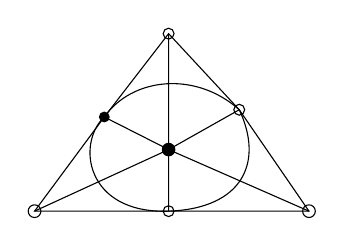
\begin{tikzpicture}[scale=1.15]
\coordinate (a) at (0,1.96);
\coordinate (b) at (-1.48,0);
\coordinate (c) at (1.55,0);
\coordinate (d) at (-0.71,1.04);
\coordinate (e) at (0.78,1.12);
\coordinate (f) at (0,0);
\coordinate (g) at (0,0.68);
\draw (a)--(d)--(b)--(f)--(c)--(e)--cycle;
\draw (a)--(g)--(f) (b)--(g)--(e) (d)--(g)--(c);
\draw (d) .. controls (-0.40,1.48) and (0.30,1.55) .. (e)
 .. controls (1.05,0.55) and (0.83,0.03) .. (f)
 .. controls (-0.92,-0.03) and (-1.02,0.75) .. (d);
\draw (a) circle (0.06) (b) circle (0.07) (c) circle (0.07)
 (e) circle (0.06) (f) circle (0.06);
\fill (d) circle (0.06) (g) circle (0.075);
\end{tikzpicture}
}
\end{minipage}
\end{center}
\noindent{\small\textit{Семь точек сохраняют две закрашенные и пять контурных отметок дипломатического рисунка. Подписи векторов не добавлены.}}
